\documentclass[12pt]{article}
\usepackage[margin=1in]{geometry}
\usepackage{float}
\usepackage{multicol}
\usepackage{lmodern}
\usepackage{amssymb,amsmath}
\usepackage{ifxetex,ifluatex}
\usepackage{fixltx2e} % provides \textsubscript
\ifnum 0\ifxetex 1\fi\ifluatex 1\fi=0 % if pdftex
  \usepackage[T1]{fontenc}
  \usepackage[utf8]{inputenc}
\else % if luatex or xelatex
  \ifxetex
    \usepackage{mathspec}
    \usepackage{xltxtra,xunicode}
  \else
    \usepackage{fontspec}
  \fi
  \defaultfontfeatures{Mapping=tex-text,Scale=MatchLowercase}
  \newcommand{\euro}{€}
\fi
% use upquote if available, for straight quotes in verbatim environments
\IfFileExists{upquote.sty}{\usepackage{upquote}}{}
% use microtype if available
\IfFileExists{microtype.sty}{%
\usepackage{microtype}
\UseMicrotypeSet[protrusion]{basicmath} % disable protrusion for tt fonts
}{}
\usepackage{longtable,booktabs}
\usepackage{graphicx}
\makeatletter
\def\maxwidth{\ifdim\Gin@nat@width>\linewidth\linewidth\else\Gin@nat@width\fi}
\def\maxheight{\ifdim\Gin@nat@height>\textheight\textheight\else\Gin@nat@height\fi}
\makeatother
% Scale images if necessary, so that they will not overflow the page
% margins by default, and it is still possible to overwrite the defaults
% using explicit options in \includegraphics[width=4in][width, height, ...]{}
\setkeys{Gin}{width=\maxwidth,height=\maxheight,keepaspectratio}
\ifxetex
  \usepackage[setpagesize=false, % page size defined by xetex
              unicode=false, % unicode breaks when used with xetex
              xetex]{hyperref}
\else
  \usepackage[unicode=true]{hyperref}
\fi
\hypersetup{breaklinks=true,
            bookmarks=true,
            pdfauthor={Brandon LeBeau},
            pdftitle={PSQF 4143: Section 4},
            colorlinks=true,
            citecolor=blue,
            urlcolor=blue,
            linkcolor=magenta,
            pdfborder={0 0 0}}
\urlstyle{same}  % don't use monospace font for urls
\setlength{\parindent}{0pt}
\setlength{\parskip}{6pt plus 2pt minus 1pt}
\setlength{\emergencystretch}{3em}  % prevent overfull lines
\setcounter{secnumdepth}{0}

\title{PSQF 4143: Section 4}
\author{Brandon LeBeau}
\date{}

\begin{document}
\maketitle

\section{Properties of the mean}\label{properties-of-the-mean}

\begin{itemize}
\itemsep1pt\parskip0pt\parsep0pt
\item
  Deviations sum to 0: Deviations are defined as \(X-\bar{X}\).
\item
  Sum of squared deviations is least for the mean (least squares
  property)
\item
  Graphically, mean is a balancing point.
\item
  In skewed distributions, mean is in the direction of the skew.
\end{itemize}

\begin{figure}[H]
\centering
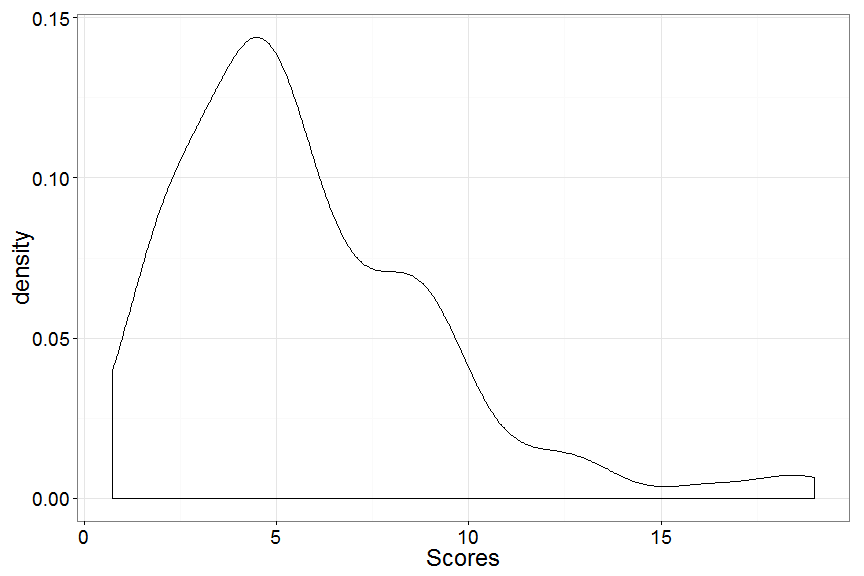
\includegraphics[width=4in]{figure/chisq-1.png}
\caption{plot of chunk chisq}
\end{figure}

\section{Variation Example}\label{variation-example}

\begin{figure}[H]
\centering
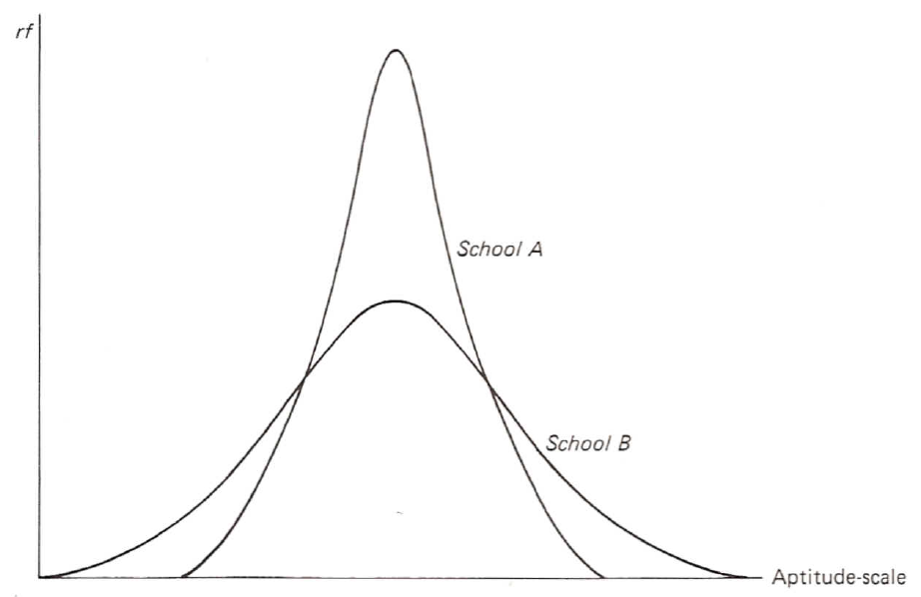
\includegraphics[width=4in]{Dispersion.png}
\caption{Variation}
\end{figure}

\section{Variation}\label{variation}

\begin{itemize}
\item
  Variability - how spread out scores are in a distribution
\item
  Central Question of Research: Why are there differences on outcomes?
\item
  Range:

  \begin{itemize}
  \itemsep1pt\parskip0pt\parsep0pt
  \item
    Upper limit of highest score (H) minus low limit of lowest score (L)
  \item
    If scores are continuous and rounded to the nearest point:
    \(Range = H - L + 1\)
  \item
    If scores are discrete: \(Range = H - L\)
  \item
    Using range as a verb: ``ACT scores ranged from 17 to 24 for the
    group''
  \end{itemize}
\item
  Interquartile Range:

  \begin{itemize}
  \itemsep1pt\parskip0pt\parsep0pt
  \item
    \(IQR = Q_{3} - Q_{1}\)
  \end{itemize}
\item
  Is the range of the sample equal to the range of the population?
\item
  Is the mean of a sample equal to the mean of the population?
\end{itemize}

\section{Expected Value}\label{expected-value}

\begin{itemize}
\itemsep1pt\parskip0pt\parsep0pt
\item
  Expected value of a statistic is the mean over all possible samples; a
  long run average.

  \begin{itemize}
  \itemsep1pt\parskip0pt\parsep0pt
  \item
    \(E(sample mean) \quad  population mean (\mu)\)
  \item
    \(E(sample range) \quad population range\)
  \end{itemize}
\item
  Range is very crude as it only takes into account two scores in our
  distribution.
\end{itemize}

\section{Semi-Interquartile Range}\label{semi-interquartile-range}

\[ Q = \frac{Q_{3} - Q_{1}}{2} \]
\[ Q = \frac{(Q_{3} - Mdn) + (Mdn - Q_{1})}{2} \]

\begin{itemize}
\itemsep1pt\parskip0pt\parsep0pt
\item
  Q is the average of the distances from the median to \(Q_{1}\) and
  \(Q_{3}\).
\end{itemize}

\section{Semi IQR Example}\label{semi-iqr-example}

\begin{figure}[H]
\centering
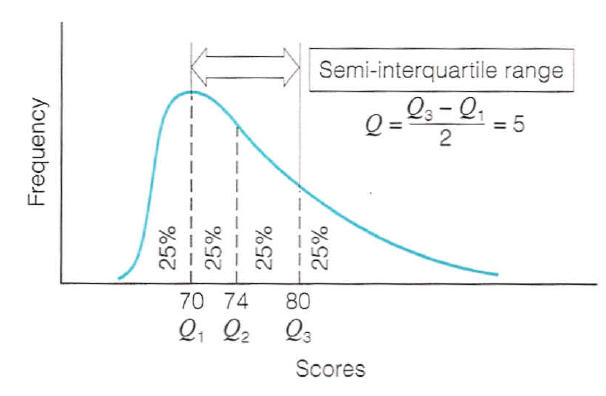
\includegraphics[width=4in]{SemiIQR.png}
\caption{Semi IQR}
\end{figure}

\begin{itemize}
\itemsep1pt\parskip0pt\parsep0pt
\item
  For non-symmetrical distributions, the semi IQR is interpreted as
  \emph{roughly} half of the scores deviate by more than 5 units from
  the median and \emph{roughly} half of the scores deviate by less than
  5 units.
\item
  For symmetrical distributions change \emph{roughly} above to
  \emph{exactly}.
\end{itemize}

\section{Variability Measures with the
Median}\label{variability-measures-with-the-median}

\begin{itemize}
\itemsep1pt\parskip0pt\parsep0pt
\item
  Average deviation from the median: \[ \frac{\sum (X_{i} - Mdn)}{n} \]

  \begin{itemize}
  \itemsep1pt\parskip0pt\parsep0pt
  \item
    Positive differences will tend to offset negative differences.
  \item
    Half of the scores are above, half are below.
  \end{itemize}
\item
  Average absolute deviation from the median:
  \[ \frac{\sum |X_{i} - Mdn|}{n} \]

  \begin{itemize}
  \itemsep1pt\parskip0pt\parsep0pt
  \item
    Uses all scores in the distribution
  \item
    Influenced by extreme scores
  \item
    Not too bad as an index of variability
  \item
    One problem is that absolute values are difficult mathematically
  \end{itemize}
\end{itemize}

\section{Variability Measures with the
Mean}\label{variability-measures-with-the-mean}

\begin{itemize}
\itemsep1pt\parskip0pt\parsep0pt
\item
  Average deviation from the mean:
  \[ \frac{\sum (X_{i} - \bar{X})}{n} \]

  \begin{itemize}
  \itemsep1pt\parskip0pt\parsep0pt
  \item
    No Good, why?
  \end{itemize}
\item
  Average absolute deviation from the mean:
  \[ \frac{\sum |X_{i} - \bar{X}|}{n} \]

  \begin{itemize}
  \itemsep1pt\parskip0pt\parsep0pt
  \item
    Not too bad as an index of variability
  \item
    One problem is that absolute values are difficult mathematically
  \item
    For more advanced statistical techniques, this will become a
    problem.
  \end{itemize}
\item
  Average squared deviations from the mean:
  \[ \frac{\sum (X_{i} - \bar{X})^2}{n} \]

  \begin{itemize}
  \itemsep1pt\parskip0pt\parsep0pt
  \item
    This is formally called the variance
  \item
    This is a very important statistical measure and the most used
    measure of variability.
  \end{itemize}
\end{itemize}

\section{Variance}\label{variance}

\begin{itemize}
\itemsep1pt\parskip0pt\parsep0pt
\item
  Sample Variance:\\\[ s^2 = \frac{\sum (X - \bar{X})^2}{n} \]
\item
  Population Variance:\\\[ \sigma^2 = \frac{\sum (X - \mu)^2}{N} \]

  \begin{itemize}
  \itemsep1pt\parskip0pt\parsep0pt
  \item
    Sum of Squares (SS) = \(\sum(X-\mu)^2\)
  \item
    Mean Squares (MS) = variance or \(\sigma^2\)
  \end{itemize}
\item
  Interpreted as the average \textbf{squared} distance from the mean.
\item
  Too bad the variance is interpreted in terms of squared units.
\end{itemize}

\section{Example}\label{example}

X\\3 4 5 6 7

\section{Standard Deviation}\label{standard-deviation}

\begin{itemize}
\itemsep1pt\parskip0pt\parsep0pt
\item
  To convert away from squared units, simply take the square root of the
  variance.
\item
  Sample SD:
  \[ s^2 = \sqrt{s^2} = \sqrt{\frac{\sum (X - \bar{X})^2}{n}} \]
\item
  Population SD:
  \[ \sigma^2 = \sqrt{\sigma^2} = \sqrt{\frac{\sum (X - \mu)^2}{n}} \]
\item
  The SD is interpreted as the average deviation score from the mean.
\end{itemize}

\section{Standard Deviation
Properties}\label{standard-deviation-properties}

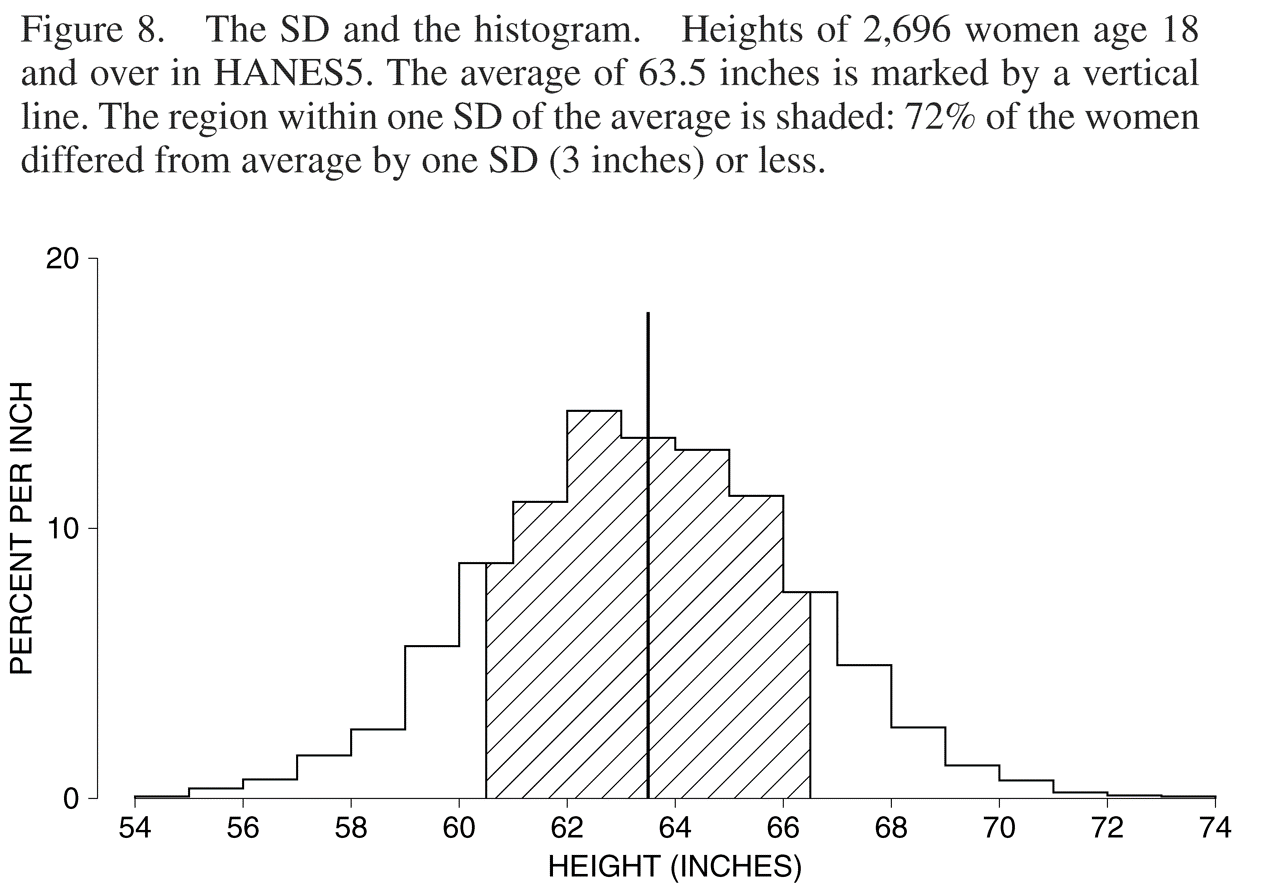
\includegraphics[width=3.5in]{sd_norm.png} 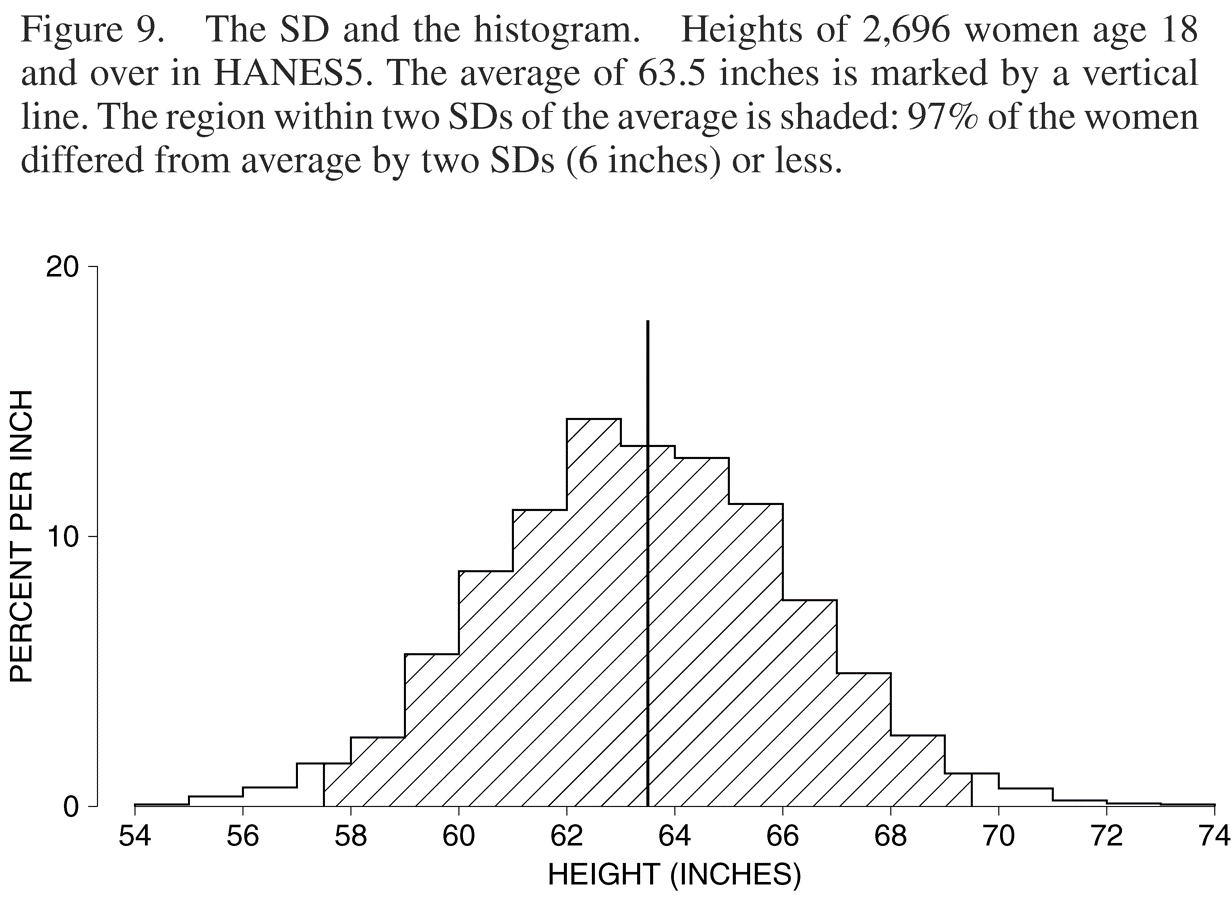
\includegraphics[width=3.5in]{sd_norm2.png}

\section{Computational Formulas}\label{computational-formulas}

\begin{itemize}
\itemsep1pt\parskip0pt\parsep0pt
\item
  Variance:
  \[ s^2 = \frac{\sum X_{i}^{2}}{n} - \left(\frac{\sum X_{i}}{n}\right)^2 = \frac{\sum X_{i}^{2}}{n} - \bar{X}^2 \]
\item
  SD:
  \[ s = \sqrt{\frac{\sum X_{i}^{2}}{n} - \left(\frac{\sum X_{i}}{n}\right)^2} = \sqrt{\frac{\sum X_{i}^{2}}{n} - \bar{X}^2} \]
\end{itemize}

\section{Calculate SD for Grouped Freq.
Dist.}\label{calculate-sd-for-grouped-freq.-dist.}

\[ s = \sqrt{\frac{\sum f_{j}X_{j}^{2}}{n} - \left(\frac{\sum f_{j}X_{j}}{n}\right)^2} = \sqrt{\frac{\sum f_{j}X_{j}^{2}}{n} - \bar{X}^2} \]
- \(f_{j}\) is the frequency of interval \(j\). - \(X_{j}\) is the
midpoint of interval \(j\).

\section{Example}\label{example-1}

\begin{longtable}[c]{@{}rrrr@{}}
\toprule
X & \(f_{j}\) & \(X_{j}\) & \(f_{j}*X_{j}\)\tabularnewline
\midrule
\endhead
1 - 4 & 3 & 2.5 & 7.5\tabularnewline
5 - 8 & 4 & 6.5 & 26\tabularnewline
9 - 12 & 8 & 10.5 & 84\tabularnewline
13 - 16 & 15 & 14.5 & 217.5\tabularnewline
17 - 20 & 28 & 18.5 & 518\tabularnewline
21 - 24 & 12 & 22.5 & 270\tabularnewline
25 - 28 & 14 & 26.5 & 371\tabularnewline
29 - 32 & 10 & 30.5 & 305\tabularnewline
33 - 36 & 6 & 34.5 & 207\tabularnewline
\bottomrule
\end{longtable}

\section{Relationship between Q and
s}\label{relationship-between-q-and-s}

\begin{figure}[H]
\centering
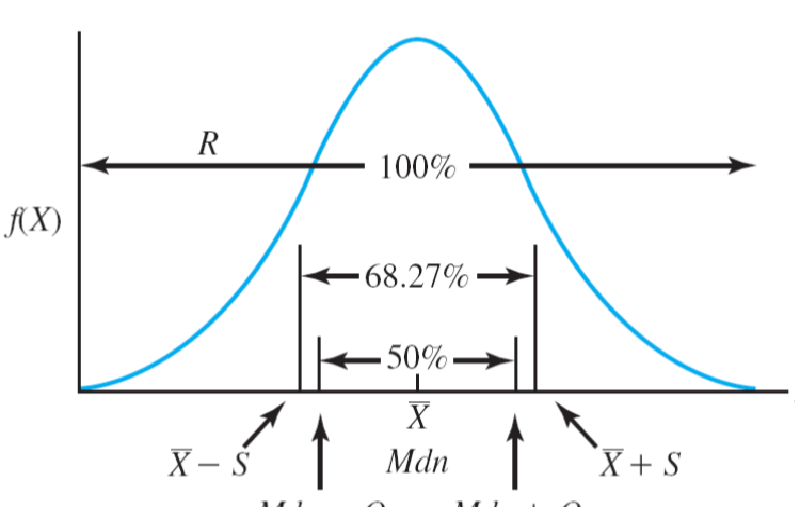
\includegraphics[width=4in]{QvsS.png}
\caption{Q vs S}
\end{figure}

\section{Q \& s with skewed
distributions}\label{q-s-with-skewed-distributions}

\begin{figure}[H]
\centering
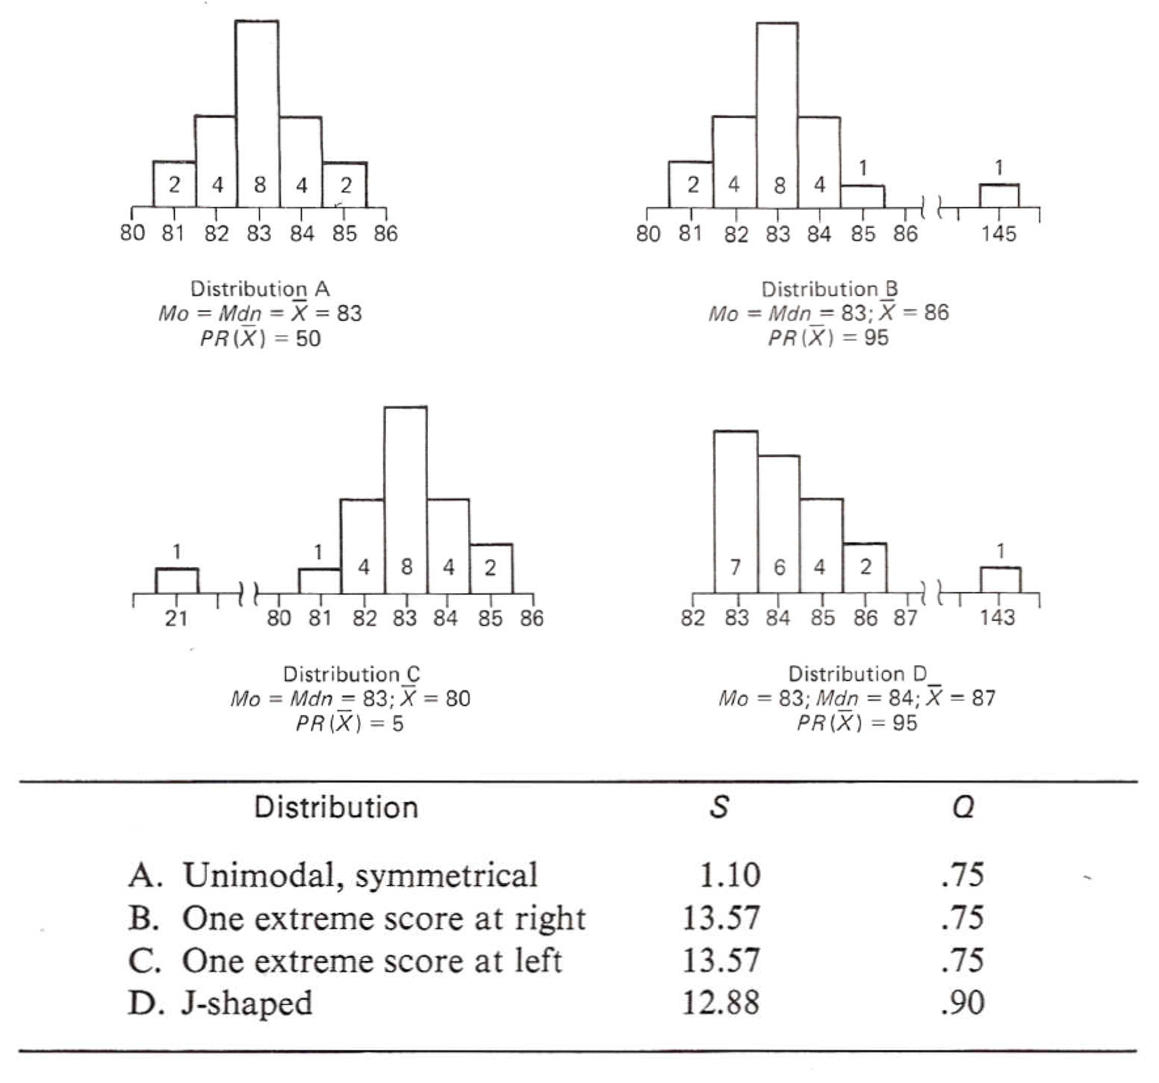
\includegraphics[width=4in]{skew_sd.png}
\caption{Q vs S}
\end{figure}

\section{Income Example}\label{football-coaches-salary}

\begin{figure}[H]
\centering
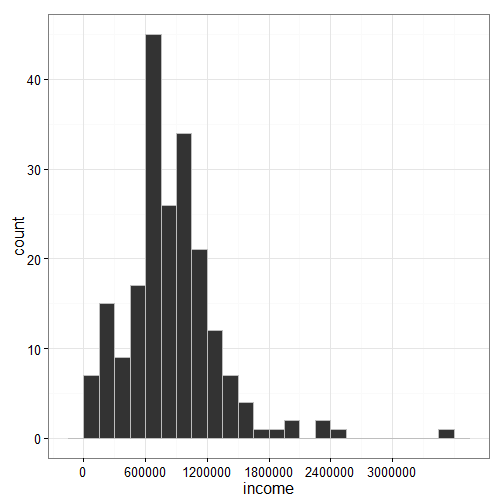
\includegraphics[width=4in]{figure/salary-1.png}
\caption{plot of chunk salary}
\end{figure}

\section{Properties of Variability
Measures}\label{properties-of-variability-measures}

\begin{itemize}
\itemsep1pt\parskip0pt\parsep0pt
\item
  Standard Deviation (Variance):

  \begin{itemize}
  \itemsep1pt\parskip0pt\parsep0pt
  \item
    A distance measure
  \item
    Preferred measure for symmetric quantitative variables
  \item
    Commonly reported with the mean
  \item
    Best sample stability
  \item
    Widely used in advanced statistical procedures - mathematically
    tractable
  \item
    Every score affects value
  \item
    Fairly sensitive to extreme scores
  \item
    Not appropriate for qualitative variables
  \end{itemize}
\item
  Semi-interquartile Range:

  \begin{itemize}
  \itemsep1pt\parskip0pt\parsep0pt
  \item
    A distance measure
  \item
    Commonly reported with the median
  \item
    Sensitive to the number and not to the value of scores above or
    below Q3 and Q1 respectively
  \item
    Appropriate for open-ended distributions
  \item
    More sample fluctuation than SD
  \item
    Rarely used in advanced statistical procedures - less mathematically
    tractable
  \end{itemize}
\item
  Range:

  \begin{itemize}
  \itemsep1pt\parskip0pt\parsep0pt
  \item
    A distance measure
  \item
    Simplest measure for quantitative variables
  \item
    Highly influenced by sample fluctuations
  \item
    Dependent on sample size
  \item
    rarely used in advanced statistical procedures - less mathematically
    tractable
  \end{itemize}
\end{itemize}

\section{Measures of Variability
Uses}\label{measures-of-variability-uses}

\begin{enumerate}
\def\labelenumi{\arabic{enumi}.}
\itemsep1pt\parskip0pt\parsep0pt
\item
  Describe Distributions
\item
  Compare Distributions
\item
  Study the accuracy of certain measuring procedures

  \begin{itemize}
  \itemsep1pt\parskip0pt\parsep0pt
  \item
    Consistency of raters rating figure skaters.
  \item
    Estimate the population mean IQ of children aged 3 to 15.
  \end{itemize}
\end{enumerate}

\section{Describing Distributions}\label{describing-distributions}

\begin{itemize}
\itemsep1pt\parskip0pt\parsep0pt
\item
  Used in conjunction with a measure of central tendency, variability
  helps us understand a distribution of scores.

  \begin{itemize}
  \itemsep1pt\parskip0pt\parsep0pt
  \item
    Examples:

    \begin{itemize}
    \itemsep1pt\parskip0pt\parsep0pt
    \item
      Consider a unimodal symmetrical distribution:
    \item
      \(Mdn = 50\), \(Q = 10\).
    \item
      \(Mean = 38\), \(SD = 6\).
    \end{itemize}
  \end{itemize}
\end{itemize}

\section{Comparing Distributions}\label{comparing-distributions}

\begin{itemize}
\itemsep1pt\parskip0pt\parsep0pt
\item
  If two distributions have the same score scale, then a direct
  comparison of variability is possible.
\item
  Cannot compare when scales are different:

  \begin{itemize}
  \itemsep1pt\parskip0pt\parsep0pt
  \item
    Example:

    \begin{itemize}
    \itemsep1pt\parskip0pt\parsep0pt
    \item
      SAT: ranges from 200 to 800, \(SD_{SAT} = 100\)
    \item
      ACT: ranges from 1 to 36, \(SD_{ACT} = 5\)
    \end{itemize}
  \end{itemize}
\end{itemize}

\section{Accuracy of Measuring
Procedures}\label{accuracy-of-measuring-procedures}

\begin{itemize}
\itemsep1pt\parskip0pt\parsep0pt
\item
  Roughly 60 million children in the US. aged 3 to 15.
\item
  Not practical to measure the IQ of every child
\item
  Settle for taking a sample of 1000 children and measure the IQ of each
\item
  Use the sample mean as an estimate of the population mean
\item
  How good is the estimate?

  \begin{itemize}
  \itemsep1pt\parskip0pt\parsep0pt
  \item
    More complicated because the population mean is unknown
  \end{itemize}
\end{itemize}

\section{Population}\label{population}

\begin{figure}[H]
\centering
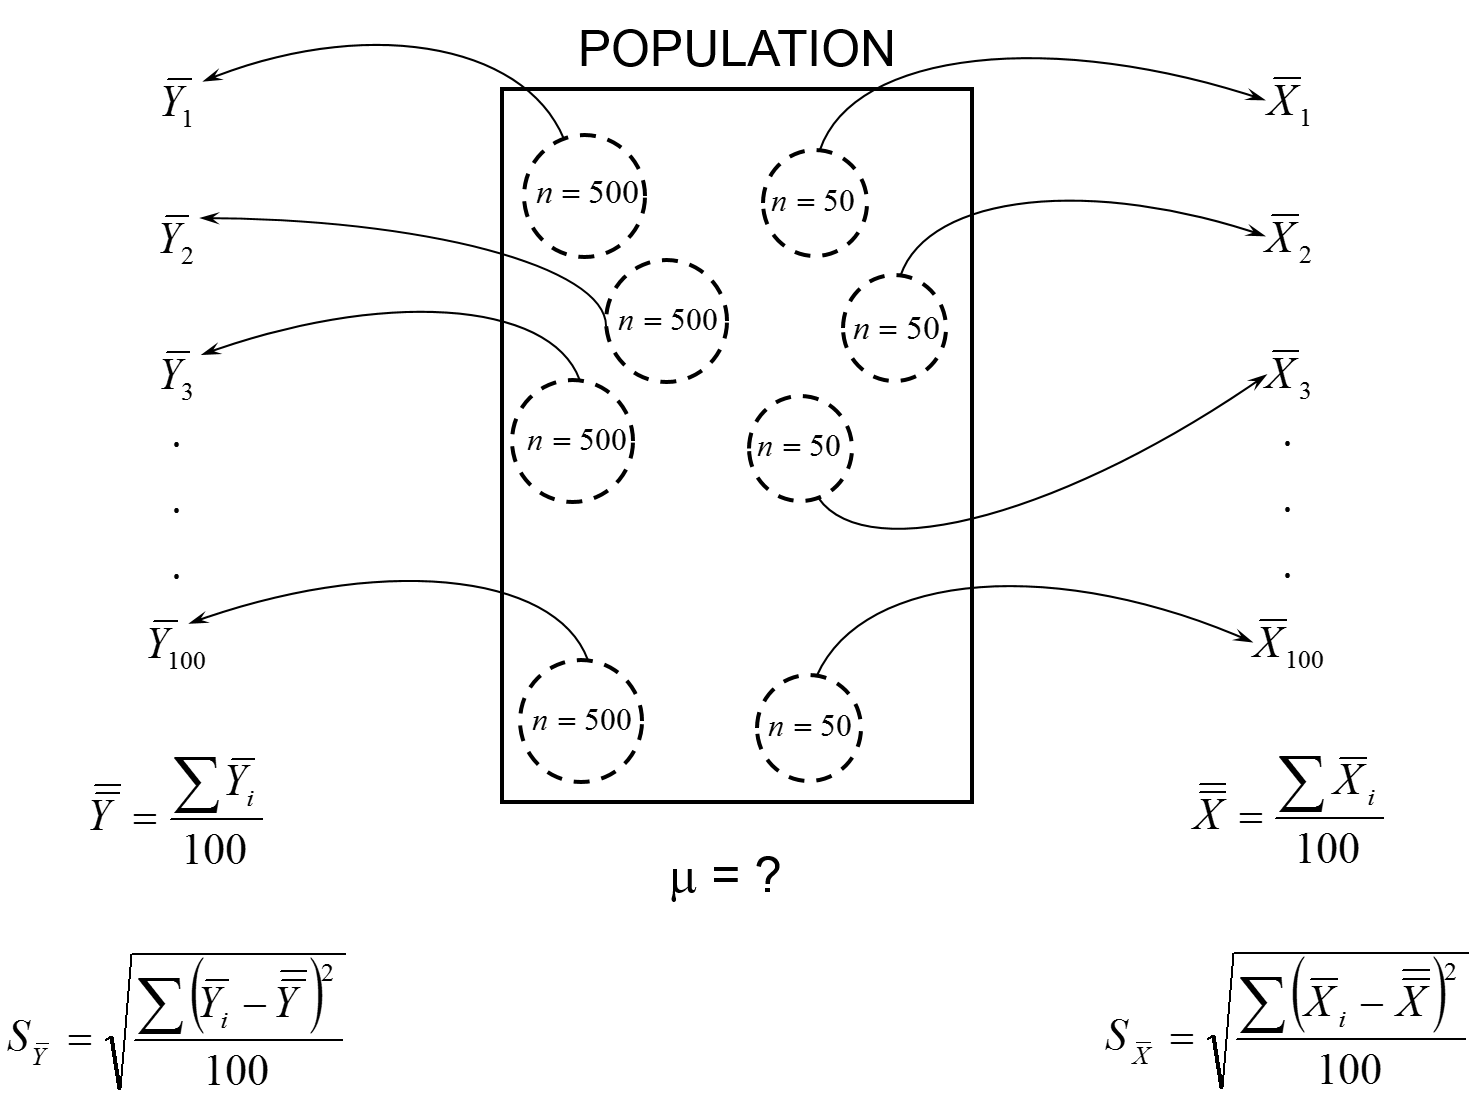
\includegraphics[width=4in]{popSDsize.png}
\caption{Popsamp}
\end{figure}

\section{Standard Deviation 3}\label{standard-deviation-3}

\begin{itemize}
\itemsep1pt\parskip0pt\parsep0pt
\item
  Problem:

  \begin{itemize}
  \itemsep1pt\parskip0pt\parsep0pt
  \item
    If we use the formula for the population on the sample, the variance
    for the sample is slightly too small - samples are closer to the
    sample mean than to the population mean. Recall that sum of squared
    deviations was smallest for the sample mean.
  \end{itemize}
\item
  Solution:

  \begin{itemize}
  \itemsep1pt\parskip0pt\parsep0pt
  \item
    Instead of dividing by \(n\), divide by \(n-1\).
  \end{itemize}
\end{itemize}

\section{Standard Deviations for
Samples}\label{standard-deviations-for-samples}

\begin{itemize}
\itemsep1pt\parskip0pt\parsep0pt
\item
  Variance: \[ s^2 = \frac{\sum (X - \bar{X})^2}{n - 1} \]
\item
  Standard Deviation:
  \[ s = \sqrt{s^2} = \sqrt{\frac{\sum (X - \bar{X})^2}{n - 1}} \]
\end{itemize}

\section{Standard Deviations for Samples
2}\label{standard-deviations-for-samples-2}

\begin{itemize}
\itemsep1pt\parskip0pt\parsep0pt
\item
  By using \(n - 1\) instead of \(n\), the expected value of the sample
  variance is the population variance. More formally:
  \[ E(s^2) = \sigma^2 \]
\item
  In words, the long run average from every possible sample from the
  population would now equal the population variance.
\end{itemize}

\section{Index of Dispersion}\label{index-of-dispersion}

\[ D = \frac{c\left( n^2 - \sum n_{j}^{2} \right)}{n^2 (c - 1)} \]

\begin{itemize}
\itemsep1pt\parskip0pt\parsep0pt
\item
  c is the number of categories
\item
  n is the total number of observations
\item
  \(n_{j}\) is the number of observations in category \(j\)
\end{itemize}

\section{Index of Dispersion Example}\label{index-of-dispersion-example}

\begin{figure}[H]
\centering
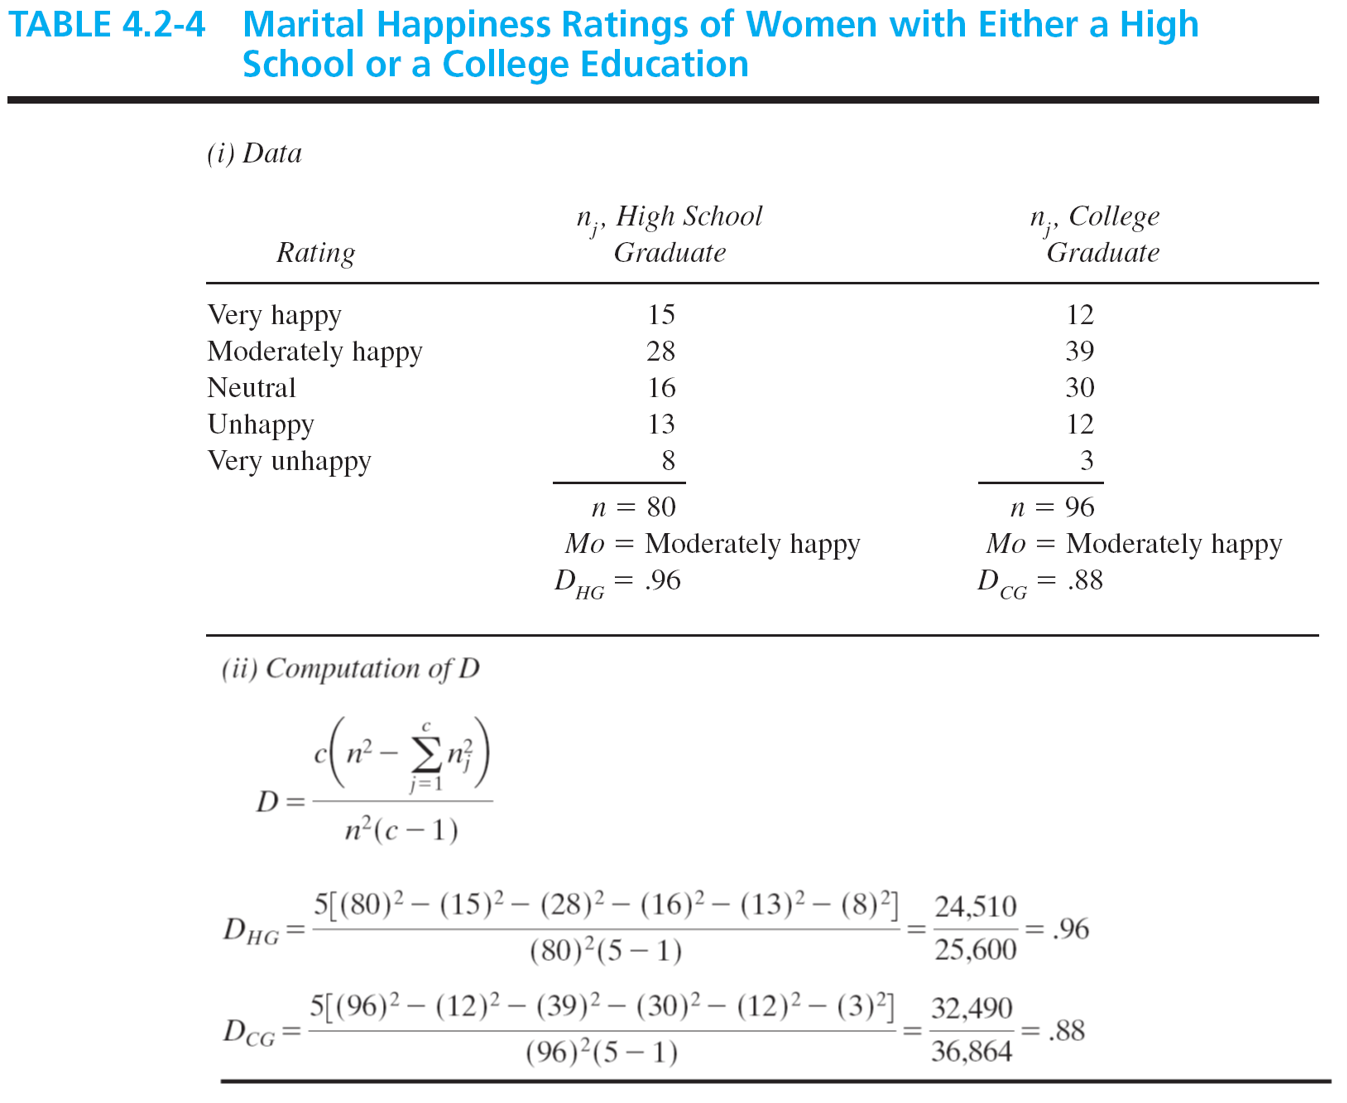
\includegraphics[width=4in]{indexdispersion.png}
\caption{Dispersion}
\end{figure}

\section{Skewness}\label{skewness}

\[Sk = \frac{\sum \left(X_{i} - \bar{X}\right)^3}{n s^3_{X}} \] -
\(Sk = 0\), symmetrical - \(Sk > 0\), positively skewed - \(Sk < 0\),
negatively skewed

\section{Kurtosis}\label{kurtosis}

\[Kur = \frac{\sum \left(X_{i} - \bar{X}\right)^4}{n s^4_{X}} - 3 \] -
\(Kur = 0\), mesokurtic - \(Kur > 0\), leptokurtic - \(Kur < 0\),
platykurtic

\section{Distribution Differences}\label{distribution-differences}

\begin{figure}[H]
\centering
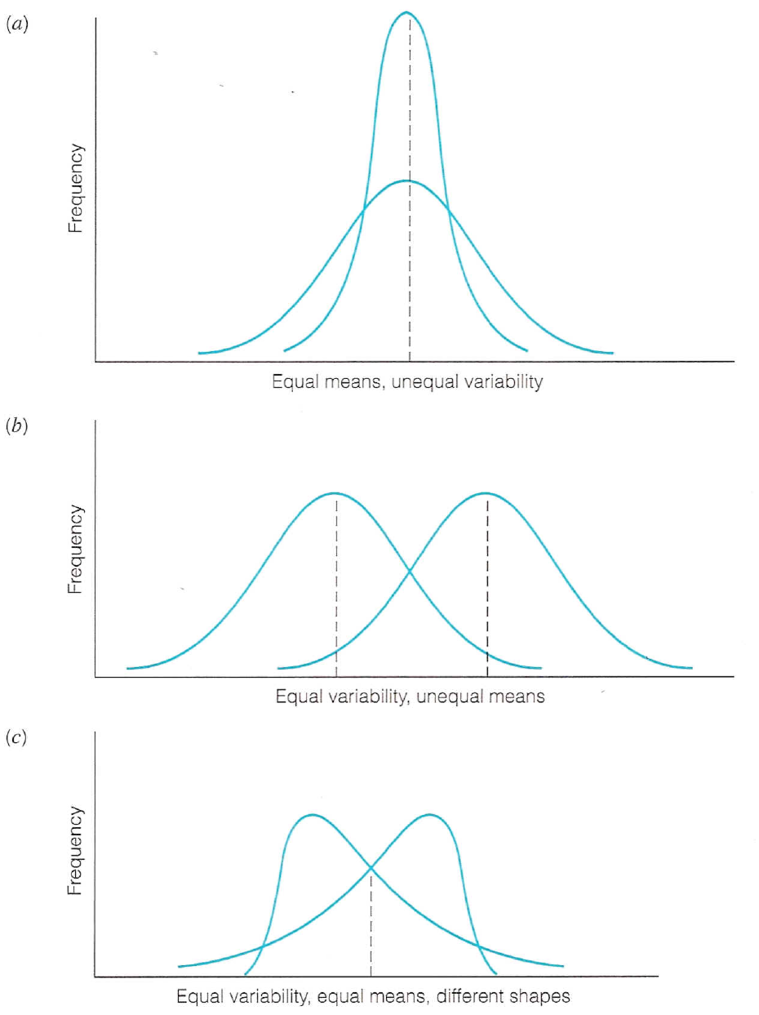
\includegraphics[width=4in]{distributiondiff.png}
\caption{Dist Diff}
\end{figure}

\section{Boxplot}\label{boxplot}

\begin{itemize}
\itemsep1pt\parskip0pt\parsep0pt
\item
  These are sometimes called a box and whisker plot
\end{itemize}

\begin{figure}[H]
\centering
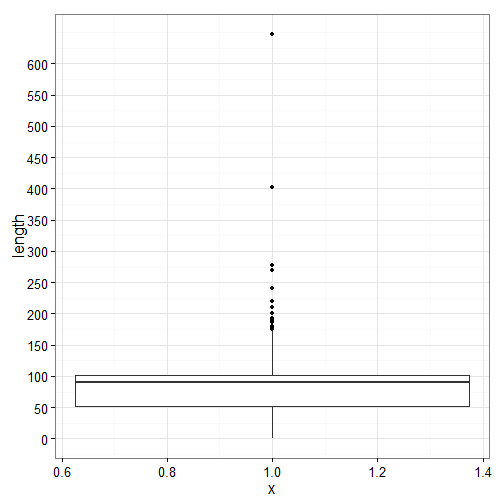
\includegraphics[width=3.5in]{figure/boxplot-1.png}
\caption{plot of chunk boxplot}
\end{figure}

\section{Boxplots by group}\label{boxplots-by-group}

\begin{figure}[H]
\centering
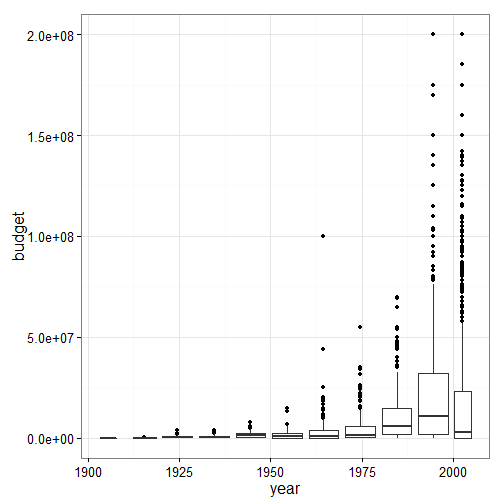
\includegraphics[width=3.5in]{figure/boxgroup-1.png}
\caption{plot of chunk boxgroup}
\end{figure}

\end{document}
